% pipeline_v55_workflow.tex -- sPHENIX TPC detached simulation pipeline, v5.5
% (field-in-digitization). Single source for both pipeline_v55_workflow.pdf and
% .svg. Successor to pipeline_detachment.svg (the detachment-era record, kept).
% Build:  pdflatex pipeline_v55_workflow.tex
%         dvisvgm --pdf pipeline_v55_workflow.pdf   (SVG twin)
% Every number here is traceable to pp_pipeline.sh (VER=v55), PIPELINE.md's
% v5.5 entries, island_post/production_manifest.txt, or a side-review re-run.
\documentclass[border=8pt]{standalone}
\usepackage[T1]{fontenc}
\usepackage{helvet}
\usepackage{courier}
\renewcommand{\familydefault}{\sfdefault}
\usepackage{array}
\usepackage{xcolor}
\usepackage{tikz}
\usetikzlibrary{arrows,positioning,calc}

% ---- palette (inherited from pipeline_detachment.svg) ----
\definecolor{ink}{HTML}{1C2733}
\definecolor{sub}{HTML}{51616F}
\definecolor{rule}{HTML}{C3CFDA}
\definecolor{lane}{HTML}{EDF1F6}
\definecolor{artf}{HTML}{E3F1F6}
\definecolor{arts}{HTML}{0E7C9C}
\definecolor{good}{HTML}{2F7D50}
\definecolor{goodf}{HTML}{E8F3EC}
\definecolor{warn}{HTML}{9A6B00}
\definecolor{warnf}{HTML}{FAF0D7}
\definecolor{fieldc}{HTML}{A8532A}
\definecolor{fieldf}{HTML}{FBEDE3}

\newcommand{\eyebrow}[1]{{\scriptsize\bfseries\color{sub}#1}}
\newcommand{\ctitle}[1]{{\small\bfseries\color{ink}#1}}
\newcommand{\m}[1]{{\ttfamily\footnotesize #1}}
\newcommand{\bd}[1]{\textbf{#1}}
\newcommand{\bul}{{\color{sub}\textbullet}\;}
% never hyphenate: broken words across a node's width read as layout noise
\hyphenpenalty=10000 \exhyphenpenalty=10000 \tolerance=9999 \emergencystretch=2em
\renewcommand{\arraystretch}{1.12}

\begin{document}
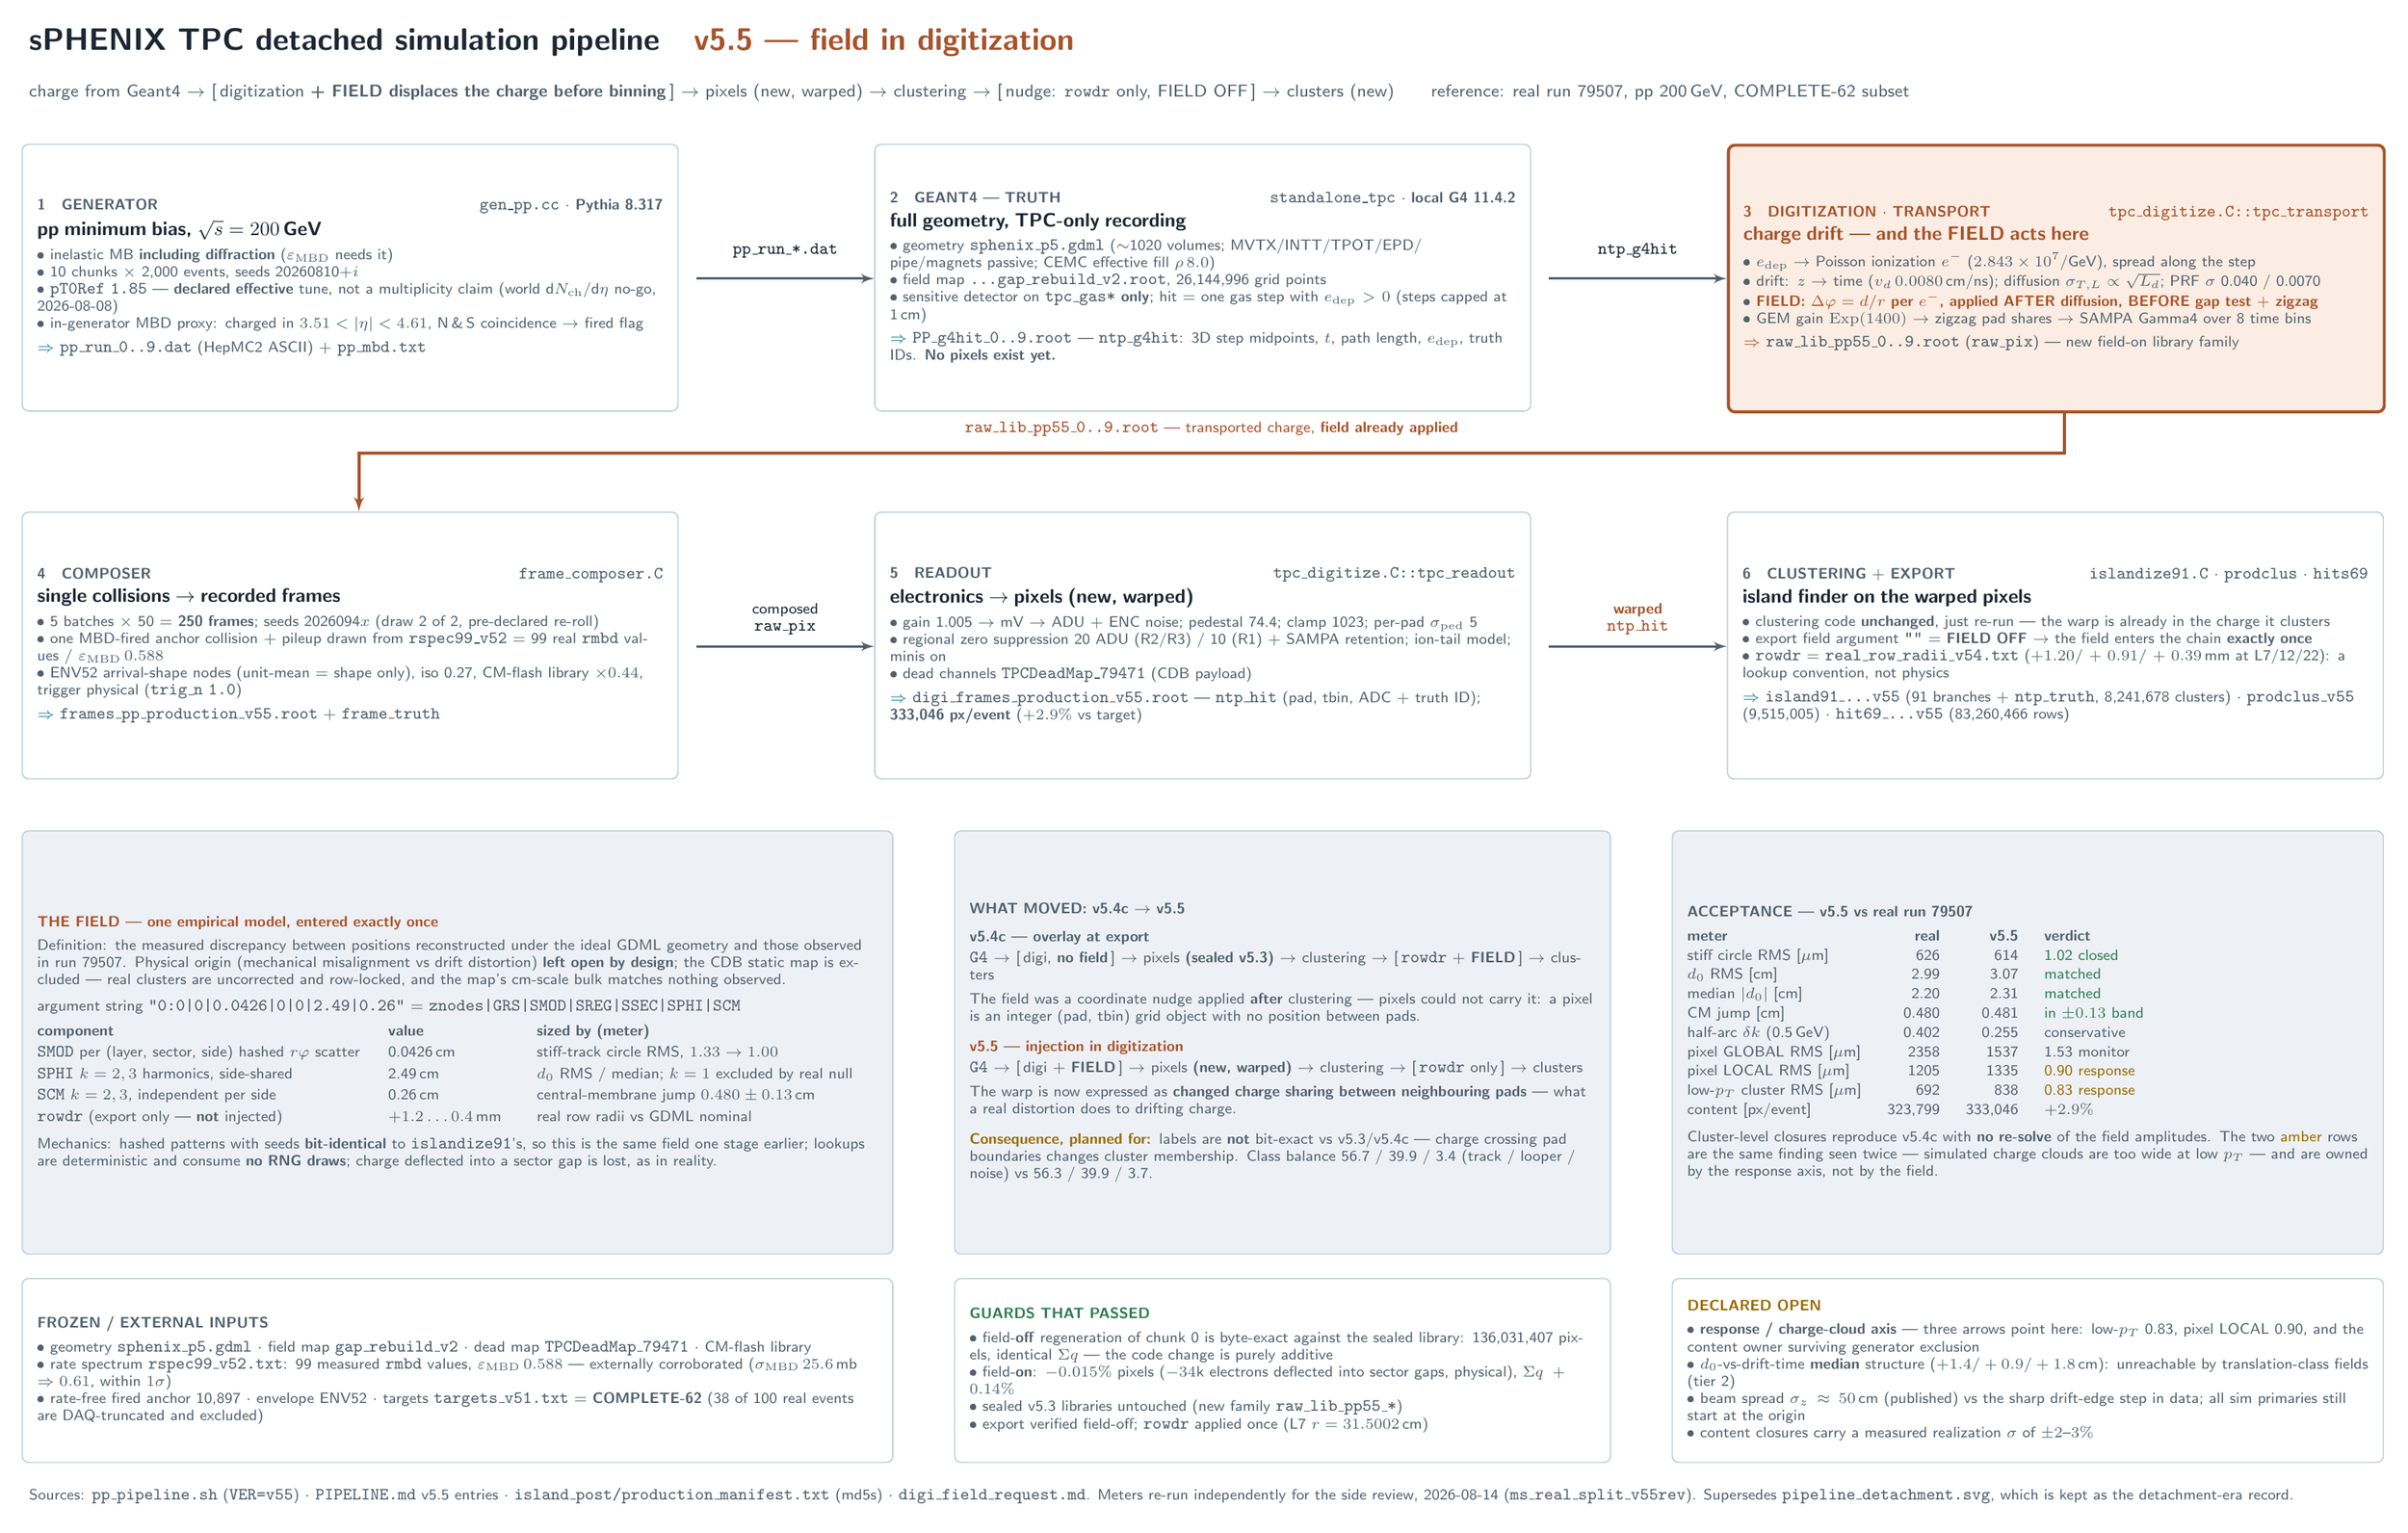
\begin{tikzpicture}[
  font=\scriptsize\color{sub},
  stage/.style={draw=rule, line width=0.6pt, fill=white, rounded corners=3pt,
                text width=10.2cm, align=left, inner sep=7pt, anchor=north west,
                minimum height=4.35cm},
  fstage/.style={stage, draw=fieldc, line width=1.4pt, fill=fieldf},
  panel/.style={draw=rule, line width=0.6pt, fill=lane, rounded corners=3pt,
                align=left, inner sep=7pt, anchor=north west},
  rail/.style={draw=rule, line width=0.6pt, fill=white, rounded corners=3pt,
               align=left, inner sep=7pt, anchor=north west},
  flow/.style={draw=sub, line width=1.1pt, ->, >=latex'},
  fflow/.style={draw=fieldc, line width=1.3pt, ->, >=latex'},
  obj/.style={fill=white, inner sep=1.5pt, align=center, text=ink}
]

% ================= title =================
\node[anchor=north west, text=ink] at (0.6,26.9)
  {\fontsize{15}{17}\selectfont\bfseries sPHENIX TPC detached simulation pipeline\quad
   \fontsize{15}{17}\selectfont\color{fieldc}v5.5 --- field in digitization};
\node[anchor=north west, text=sub] at (0.6,26.0)
  {\footnotesize charge from Geant4 $\to$ [\,digitization \bd{+ FIELD displaces the charge
   before binning}\,] $\to$ pixels (new, warped) $\to$ clustering $\to$
   [\,nudge: \m{rowdr} only, FIELD OFF\,] $\to$ clusters (new)\qquad
   reference: real run 79507, pp 200\,GeV, COMPLETE-62 subset};

% ================= ROW A =================
\node[stage] (c1) at (0.6,24.9) {%
  \eyebrow{1 \ \ GENERATOR}\hfill\eyebrow{\m{gen\_pp.cc} $\cdot$ Pythia 8.317}\\[2pt]
  \ctitle{pp minimum bias, $\sqrt{s}=200$\,GeV}\\[3pt]
  \bul inelastic MB \bd{including diffraction} ($\varepsilon_{\rm MBD}$ needs it)\\
  \bul 10 chunks $\times$ 2{,}000 events, seeds 20260810$+i$\\
  \bul \m{pT0Ref 1.85} --- \bd{declared effective} tune, not a multiplicity
       claim (world d$N_{\rm ch}$/d$\eta$ no-go, 2026-08-08)\\
  \bul in-generator MBD proxy: charged in $3.51<|\eta|<4.61$,
       N\,\&\,S coincidence $\to$ fired flag\\[3pt]
  {\color{arts}$\Rightarrow$} \m{pp\_run\_0..9.dat} (HepMC2 ASCII) $+$ \m{pp\_mbd.txt}};

\node[stage] (c2) at (14.5,24.9) {%
  \eyebrow{2 \ \ GEANT4 --- TRUTH}\hfill\eyebrow{\m{standalone\_tpc} $\cdot$ local G4 11.4.2}\\[2pt]
  \ctitle{full geometry, TPC-only recording}\\[3pt]
  \bul geometry \m{sphenix\_p5.gdml} ($\sim$1020 volumes; MVTX/INTT/TPOT/EPD/
       pipe/magnets passive; CEMC effective fill $\rho\,8.0$)\\
  \bul field map \m{...gap\_rebuild\_v2.root}, 26{,}144{,}996 grid points\\
  \bul sensitive detector on \m{tpc\_gas*} \bd{only}; hit $=$ one gas step
       with $e_{\rm dep}>0$ (steps capped at 1\,cm)\\[3pt]
  {\color{arts}$\Rightarrow$} \m{PP\_g4hit\_0..9.root} --- \m{ntp\_g4hit}: 3D step
  midpoints, $t$, path length, $e_{\rm dep}$, truth IDs. \bd{No pixels exist yet.}};

\node[fstage] (c3) at (28.4,24.9) {%
  \eyebrow{\color{fieldc}3 \ \ DIGITIZATION $\cdot$ TRANSPORT}\hfill
  \eyebrow{\color{fieldc}\m{tpc\_digitize.C::tpc\_transport}}\\[2pt]
  \ctitle{\color{fieldc}charge drift --- and the FIELD acts here}\\[3pt]
  \bul $e_{\rm dep}\to$ Poisson ionization $e^-$ ($2.843\times10^{7}$/GeV),
       spread along the step\\
  \bul drift: $z\to$ time ($v_d\,0.0080$\,cm/ns); diffusion
       $\sigma_{T,L}\propto\sqrt{L_d}$; PRF $\sigma$ 0.040 / 0.0070\\
  \bul \bd{\color{fieldc}FIELD: $\Delta\varphi=d/r$ per $e^-$, applied AFTER
       diffusion, BEFORE gap test $+$ zigzag}\\
  \bul GEM gain ${\rm Exp}(1400)$ $\to$ zigzag pad shares $\to$ SAMPA
       Gamma4 over 8 time bins\\[3pt]
  {\color{fieldc}$\Rightarrow$} \m{raw\_lib\_pp55\_0..9.root} (\m{raw\_pix}) ---
  new field-on library family};

% ================= ROW B =================
\node[stage] (c4) at (0.6,18.9) {%
  \eyebrow{4 \ \ COMPOSER}\hfill\eyebrow{\m{frame\_composer.C}}\\[2pt]
  \ctitle{single collisions $\to$ recorded frames}\\[3pt]
  \bul 5 batches $\times$ 50 $=$ \bd{250 frames}; seeds 2026094$x$
       (draw 2 of 2, pre-declared re-roll)\\
  \bul one MBD-fired anchor collision $+$ pileup drawn from
       \m{rspec99\_v52} $=$ 99 real \m{rmbd} values $/\ \varepsilon_{\rm MBD}\,0.588$\\
  \bul ENV52 arrival-shape nodes (unit-mean $=$ shape only), iso 0.27,
       CM-flash library $\times0.44$, trigger physical (\m{trig\_n 1.0})\\[3pt]
  {\color{arts}$\Rightarrow$} \m{frames\_pp\_production\_v55.root} $+$ \m{frame\_truth}};

\node[stage] (c5) at (14.5,18.9) {%
  \eyebrow{5 \ \ READOUT}\hfill\eyebrow{\m{tpc\_digitize.C::tpc\_readout}}\\[2pt]
  \ctitle{electronics $\to$ \bd{pixels (new, warped)}}\\[3pt]
  \bul gain 1.005 $\to$ mV $\to$ ADU $+$ ENC noise; pedestal 74.4;
       clamp 1023; per-pad $\sigma_{\rm ped}$ 5\\
  \bul regional zero suppression 20 ADU (R2/R3) / 10 (R1) $+$ SAMPA
       retention; ion-tail model; minis on\\
  \bul dead channels \m{TPCDeadMap\_79471} (CDB payload)\\[3pt]
  {\color{arts}$\Rightarrow$} \m{digi\_frames\_production\_v55.root} ---
  \m{ntp\_hit} (pad, tbin, ADC $+$ truth ID); \bd{333{,}046 px/event}
  ($+2.9\%$ vs target)};

\node[stage] (c6) at (28.4,18.9) {%
  \eyebrow{6 \ \ CLUSTERING $+$ EXPORT}\hfill\eyebrow{\m{islandize91.C} $\cdot$ \m{prodclus} $\cdot$ \m{hits69}}\\[2pt]
  \ctitle{island finder on the warped pixels}\\[3pt]
  \bul clustering code \bd{unchanged}, just re-run --- the warp is already
       in the charge it clusters\\
  \bul export field argument \m{""} $=$ \bd{FIELD OFF} $\to$ the field enters
       the chain \bd{exactly once}\\
  \bul \m{rowdr} $=$ \m{real\_row\_radii\_v54.txt} ($+1.20/+0.91/+0.39$\,mm at
       L7/12/22): a lookup convention, not physics\\[3pt]
  {\color{arts}$\Rightarrow$} \m{island91\_...v55} (91 branches $+$ \m{ntp\_truth},
  8{,}241{,}678 clusters) $\cdot$ \m{prodclus\_v55} (9{,}515{,}005) $\cdot$
  \m{hit69\_...v55} (83{,}260{,}466 rows)};

% ---- flow arrows, row A ----
\draw[flow] (11.6,22.7) -- (14.5,22.7);
\node[obj] at (13.05,23.15) {\m{pp\_run\_*.dat}};
\draw[flow] (25.5,22.7) -- (28.4,22.7);
\node[obj] at (26.95,23.15) {\m{ntp\_g4hit}};

% ---- wrap A -> B ----
\draw[fflow] (33.9,20.55) -- (33.9,19.85) -- (6.1,19.85) -- (6.1,18.9);
\node[obj, text=fieldc] at (20.0,20.25)
  {\m{raw\_lib\_pp55\_0..9.root} --- transported charge, \bd{field already applied}};

% ---- flow arrows, row B ----
\draw[flow] (11.6,16.7) -- (14.5,16.7);
\node[obj] at (13.05,17.15) {composed\\\m{raw\_pix}};
\draw[flow] (25.5,16.7) -- (28.4,16.7);
\node[obj, text=fieldc] at (26.95,17.15) {\bd{warped}\\\m{ntp\_hit}};

% ================= PANELS =================
\node[panel, text width=13.7cm, minimum height=6.9cm] (p1) at (0.6,13.7) {%
  \eyebrow{\color{fieldc}THE FIELD --- one empirical model, entered exactly once}\\[3pt]
  {\color{sub}Definition: the measured discrepancy between positions reconstructed
  under the ideal GDML geometry and those observed in run 79507. Physical origin
  (mechanical misalignment vs drift distortion) \bd{left open by design}; the CDB
  static map is excluded --- real clusters are uncorrected and row-locked, and the
  map's cm-scale bulk matches nothing observed.}\\[4pt]
  argument string \m{"0:0|0|0.0426|0|0|2.49|0.26"} $=$
  \m{znodes|GRS|SMOD|SREG|SSEC|SPHI|SCM}\\[3pt]
  \begin{tabular}{@{}>{\raggedright\arraybackslash}p{5.3cm}>{\raggedright\arraybackslash}p{2.0cm}>{\raggedright\arraybackslash}p{5.3cm}@{}}
  \bd{component} & \bd{value} & \bd{sized by (meter)}\\[1pt]
  \m{SMOD} per (layer, sector, side) hashed $r\varphi$ scatter & 0.0426\,cm
    & stiff-track circle RMS, $1.33\to1.00$\\[1pt]
  \m{SPHI} $k=2,3$ harmonics, side-shared & 2.49\,cm
    & $d_0$ RMS / median; $k=1$ excluded by real null\\[1pt]
  \m{SCM} $k=2,3$, independent per side & 0.26\,cm
    & central-membrane jump $0.480\pm0.13$\,cm\\[1pt]
  \m{rowdr} (export only --- \bd{not} injected) & $+1.2\ldots0.4$\,mm
    & real row radii vs GDML nominal\\
  \end{tabular}\\[4pt]
  {\color{sub}Mechanics: hashed patterns with seeds \bd{bit-identical} to
  \m{islandize91}'s, so this is the same field one stage earlier; lookups are
  deterministic and consume \bd{no RNG draws}; charge deflected into a sector gap
  is lost, as in reality.}};

\node[panel, text width=10.2cm, minimum height=6.9cm] (p2) at (15.8,13.7) {%
  \eyebrow{WHAT MOVED: v5.4c $\to$ v5.5}\\[5pt]
  {\bfseries\color{sub}v5.4c --- overlay at export}\\[2pt]
  \m{G4} $\to$ [\,digi, \bd{no field}\,] $\to$ pixels \bd{(sealed v5.3)}
  $\to$ clustering $\to$ [\,\m{rowdr} $+$ \bd{FIELD}\,] $\to$ clusters\\[3pt]
  {\color{sub}The field was a coordinate nudge applied \bd{after} clustering ---
  pixels could not carry it: a pixel is an integer (pad, tbin) grid object with no
  position between pads.}\\[6pt]
  {\bfseries\color{fieldc}v5.5 --- injection in digitization}\\[2pt]
  \m{G4} $\to$ [\,digi \bd{$+$ FIELD}\,] $\to$ pixels \bd{(new, warped)}
  $\to$ clustering $\to$ [\,\m{rowdr} only\,] $\to$ clusters\\[3pt]
  {\color{sub}The warp is now expressed as \bd{changed charge sharing between
  neighbouring pads} --- what a real distortion does to drifting charge.}\\[6pt]
  {\color{warn}\bd{Consequence, planned for:}} labels are \bd{not} bit-exact vs
  v5.3/v5.4c --- charge crossing pad boundaries changes cluster membership.
  Class balance 56.7 / 39.9 / 3.4 (track / looper / noise) vs 56.3 / 39.9 / 3.7.};

\node[panel, text width=11.1cm, minimum height=6.9cm] (p3) at (27.5,13.7) {%
  \eyebrow{ACCEPTANCE --- v5.5 vs real run 79507}\\[4pt]
  \begin{tabular}{@{}lrrl@{}}
  \bd{meter} & \bd{real} & \bd{v5.5} & \bd{verdict}\\
  stiff circle RMS [$\mu$m] & 626 & 614 & {\color{good}1.02 closed}\\
  $d_0$ RMS [cm] & 2.99 & 3.07 & {\color{good}matched}\\
  median $|d_0|$ [cm] & 2.20 & 2.31 & {\color{good}matched}\\
  CM jump [cm] & 0.480 & 0.481 & {\color{good}in $\pm0.13$ band}\\
  half-arc $\delta k$ (0.5\,GeV) & 0.402 & 0.255 & conservative\\
  pixel GLOBAL RMS [$\mu$m] & 2358 & 1537 & 1.53 monitor\\
  pixel LOCAL RMS [$\mu$m] & 1205 & 1335 & {\color{warn}0.90 response}\\
  low-$p_T$ cluster RMS [$\mu$m] & 692 & 838 & {\color{warn}0.83 response}\\
  content [px/event] & 323{,}799 & 333{,}046 & $+2.9\%$
  \end{tabular}\\[4pt]
  {\color{sub}Cluster-level closures reproduce v5.4c with \bd{no re-solve} of the
  field amplitudes. The two \color{warn}amber\color{sub}{} rows are the same
  finding seen twice --- simulated charge clouds are too wide at low $p_T$ ---
  and are owned by the response axis, not by the field.}};

% ================= BOTTOM RAIL =================
\node[rail, text width=13.7cm, minimum height=3.0cm] at (0.6,6.4) {%
  \eyebrow{FROZEN / EXTERNAL INPUTS}\\[3pt]
  \bul geometry \m{sphenix\_p5.gdml} $\cdot$ field map \m{gap\_rebuild\_v2}
  $\cdot$ dead map \m{TPCDeadMap\_79471} $\cdot$ CM-flash library\\
  \bul rate spectrum \m{rspec99\_v52.txt}: 99 measured \m{rmbd} values,
  $\varepsilon_{\rm MBD}\,0.588$ --- externally corroborated
  ($\sigma_{\rm MBD}\,25.6$\,mb $\Rightarrow0.61$, within $1\sigma$)\\
  \bul rate-free fired anchor 10{,}897 $\cdot$ envelope ENV52 $\cdot$ targets
  \m{targets\_v51.txt} $=$ \bd{COMPLETE-62} (38 of 100 real events are
  DAQ-truncated and excluded)};

\node[rail, text width=10.2cm, minimum height=3.0cm] at (15.8,6.4) {%
  \eyebrow{\color{good}GUARDS THAT PASSED}\\[3pt]
  \bul field-\bd{off} regeneration of chunk 0 is byte-exact against the sealed
  library: 136{,}031{,}407 pixels, identical $\Sigma q$ --- the code change is
  purely additive\\
  \bul field-\bd{on}: $-0.015\%$ pixels ($-34$k electrons deflected into sector
  gaps, physical), $\Sigma q\,+0.14\%$\\
  \bul sealed v5.3 libraries untouched (new family \m{raw\_lib\_pp55\_*})\\
  \bul export verified field-off; \m{rowdr} applied once (L7 $r=31.5002$\,cm)};

\node[rail, text width=11.1cm, minimum height=3.0cm] at (27.5,6.4) {%
  \eyebrow{\color{warn}DECLARED OPEN}\\[3pt]
  \bul \bd{response / charge-cloud axis} --- three arrows point here: low-$p_T$
  0.83, pixel LOCAL 0.90, and the content owner surviving generator exclusion\\
  \bul $d_0$-vs-drift-time \bd{median} structure ($+1.4/+0.9/+1.8$\,cm):
  unreachable by translation-class fields (tier 2)\\
  \bul beam spread $\sigma_z\approx50$\,cm (published) vs the sharp drift-edge
  step in data; all sim primaries still start at the origin\\
  \bul content closures carry a measured realization $\sigma$ of $\pm2$--$3\%$};

% ================= footer =================
\node[anchor=north west, text=sub] at (0.6,3.1) {%
  \scriptsize Sources: \m{pp\_pipeline.sh} (\m{VER=v55}) $\cdot$ \m{PIPELINE.md}
  v5.5 entries $\cdot$ \m{island\_post/production\_manifest.txt} (md5s) $\cdot$
  \m{digi\_field\_request.md}. Meters re-run independently for the side review,
  2026-08-14 (\m{ms\_real\_split\_v55rev}). Supersedes \m{pipeline\_detachment.svg},
  which is kept as the detachment-era record.};

\end{tikzpicture}
\end{document}
